\documentclass{beamer}
\usepackage{ctex, hyperref}
\usepackage[T1]{fontenc}
\usepackage{caption}
% other packages
\usepackage{latexsym,amsmath,xcolor,multicol,booktabs,calligra,threeparttable,geometry,adjustbox,makecell}
\usepackage{graphicx,pstricks,listings,stackengine}
\usepackage{ulem}
\usepackage[skins]{tcolorbox}

\author{刘斌 \inst{1} 甄洋 \inst{1} 李小帆 \inst{2}}
\title{
    规制融合对数字贸易的影响:\\
    基于WIOD数字内容行业的检验
}
\institute{
    \inst{1} 对外经济贸易大学中国WTO研究院, \\
    \inst{2} 复旦大学世界经济系
}
\usepackage{Whu}

% defs
\def\cmd#1{\texttt{\color{red}\footnotesize $\backslash$#1}}
\def\env#1{\texttt{\color{blue}\footnotesize #1}}
\definecolor{deepblue}{rgb}{0,0,0.5}
\definecolor{deepred}{rgb}{0.6,0,0}
\definecolor{deepgreen}{rgb}{0,0.5,0}
\definecolor{halfgray}{gray}{0.55}
\definecolor{lightyellow}{RGB}{255,255,204}

\lstset{
    basicstyle=\ttfamily\small,
    keywordstyle=\bfseries\color{deepblue},
    emphstyle=\ttfamily\color{deepred},    % Custom highlighting style
    stringstyle=\color{deepgreen},
    numbers=left,
    numberstyle=\small\color{halfgray},
    rulesepcolor=\color{red!20!green!20!blue!20},
    frame=shadowbox,
}

\setCJKfamilyfont{zhsong}{simsun.ttc}
\setCJKfamilyfont{zhhei}{simhei.ttf}
\newcommand{\zhsong}{\CJKfamily{zhsong}}  %中易宋体
\newcommand{\zhhei}{\CJKfamily{zhhei}}  %中易黑体

\begin{document}

\kaishu

\begin{frame}
    \titlepage
    \vfill
    \begin{center}
        \small
        吴予锐 \  2022302111417
    \end{center}
\end{frame}

\begin{frame}
    \begin{multicols}{2}
    \tableofcontents[
        sections={1-4},
        sectionstyle=show,
        subsectionstyle=show/shaded/hide,
        subsubsectionstyle=show/shaded/hide
    ]
    \columnbreak
    \tableofcontents[
        sections={5-8},
        sectionstyle=show,
        subsectionstyle=show/shaded/hide,
        subsubsectionstyle=show/shaded/hide
    ]
    \end{multicols}
\end{frame}


\section{研究背景}
\begin{frame}{研究背景}
    \centering
    \large
    \begin{itemize}
        \item 全球数字贸易高速增长。
        \item 数字贸易目前没有形成全球统一规则。
        \item 世界各经济体所主张的数字贸易规则并不一致。
    \end{itemize}
\end{frame}

\begin{frame}{研究动机}
    \begin{itemize}
        \item 较少文献研究数字贸易条款经济影响,且与数字贸易相关的文献大多仅限于政策分析和定性研究。 {\zhhei 本文较早关注规制融合与数字贸易的相关性的经验研究。}
        \item 囿于数据可获性,数字贸易的度量一直是学术界的难点。 {\zhhei 本文为计量分析提供可供检验的“干净样本”。}
        \item 国内对数字贸易规则深度的研究较少。 {\zhhei 本文对规制融合进行了较为准确的测度。} 国内外对美式和欧式模板的经验研究较少。 {\zhhei 本文构建数字贸易模板相似度指标分析二者对数字贸易影响的差异性。}
        \item 传统分析侧重规制融合通过降低贸易成本促进国际贸易。 {\zhhei 本文选取双边网络效应进行数字贸易机制分析。}
    \end{itemize}
\end{frame}


\section{研究问题}
\begin{frame}{研究问题}
    \centering
    \large
    \begin{itemize}
        \item 在全球数字贸易规则尚不完善的背景下,规制融合对数字贸易存在怎样的影响?
    \end{itemize}
\end{frame}


\section{研究内容}
\begin{frame}{研究过程}
    \begin{enumerate}
        \item 基准回归
        \begin{itemize}
            \item {\footnotesize 采用普通最小二乘回归和泊松伪极大似然估计方法进行基准回归分析}
            \item {\footnotesize 更换数字指标进行稳健性检验}
            \item {\footnotesize 采用多期倍差方法解决样本选择偏差产生的内生性问题;采用工具变量法和两阶段最小二乘方法解决模型中的反向因果问题}
        \end{itemize}
        \item 机制检验
        \begin{itemize}
            \item {\footnotesize 构建中介效应模型采用间接测度法进行普通最小二乘回归对贸易成本进行机制检验}
            \item {\footnotesize 运用双边双向网络链接作为替代变量进行中介效用分析对双边网络效应进行机制检验}
            \item {\footnotesize 运用政治制度和经济制度测算出双边制度距离对制度距离进行机制检验}
        \end{itemize}
        \item 扩展分析
        \begin{itemize}
            \item {\footnotesize 对3个数字贸易行业进行分样本回归以分析数字贸易行业的差异性}
            \item {\footnotesize 构建数字贸易美式模板相似度指标和数字贸易欧式模板相似度指标进行回归以分析美式模板与欧式模板的差异性}
        \end{itemize}
    \end{enumerate}
\end{frame}

\begin{frame}{研究发现}
    \begin{enumerate}
        \item 规制融合对数字贸易具有促进作用
        \item 规制融合对数字贸易可能的影响渠道
        \begin{itemize}
            \item 数字贸易通过降低贸易成本促进数字贸易的发展
            \item 规制融合通过增强双边网络效应进而促进数字贸易的发展
            \item 规制融合会通过降低制度距离促进数字贸易的发展
        \end{itemize}
        \item 规制融合对不同数字贸易行业产生的影响
        \begin{itemize}
            \item 对“电影、视频和电视节目制作,录音和音乐出版活动以及节目编制和广播活动”行业的数字贸易作用最大且最为显著
            \item 其次是“电信业”
            \item 最后是“计算机编程、咨询等相关活动与信息服务活动”行业
        \end{itemize}
        \item 尽管美式模板的标准更高,但相较于欧式模板,美式模板并没有表现出对数字贸易更强的促进作用
    \end{enumerate}
\end{frame}


\section{文献综述}
\begin{frame}
    \setbeamertemplate{itemize subitem}{}
    \begin{itemize}
        \item 区域贸易协定对“第一代”和“第二代”贸易的影响
        \begin{itemize}
            \item Viner(1950); Cernat(2001); 韩剑等(2018); Horn et al.(2010);盛斌和果婷(2016).
        \end{itemize}
        \item 数字贸易的概念与测定
        \begin{itemize}
            \item Weber(2010); OECD(2017).
        \end{itemize}
        \item 数字技术对传统货物贸易和服务贸易的影响
        \begin{itemize}
            \item Freund and Weinhold(2004); Choi(2010); 裴长洪和刘斌(2020); Lendle et al.(2016); Kim et al.(2017); Javier and Janos(2018).
        \end{itemize}
        \item 数字贸易规则对数字贸易的影响
        \begin{itemize}
            \item Sacha(2003); Weber(2010); 李杨等(2016); 周念利和陈寰琦(2018).
        \end{itemize}
    \end{itemize}
\end{frame}


\section{理论模型}
\begin{frame}{基本假定}
    \textbf{模型的基本假定为:}
    \begin{enumerate}
        \item 数字产品市场为垄断竞争市场,数字产品之间为不完全替代关系,替代弹性为 $\sigma$ 
        \item 每个企业 $v$ 只生产 $1$ 种数字产品,生产的产品可以同时向国内和国外市场出售
        \item $i$ 国企业进入 $j$ 国市场需要支付固定成本 $F_{ij}$ 
        \begin{itemize}
            \item 固定成本的存在使各国向其他国家或地区出口数字产品的数量由零利润条件内生决定
        \end{itemize}
        \item 劳动是企业唯一的生产投入要素,生产函数具有常数规模报酬属性
    \end{enumerate}
\end{frame}

\begin{frame}{数字贸易的需求与偏好}
    \begin{itemize}
        \item 使用垄断竞争的Dixit-Stiglitz模型和不变替代弹性(CES)效用函数可以表示\ \underline{数字产品进口国 $j$ 的代表性消费者的偏好} 为:
        \begin{gather*}
            U_j = (\sum_{i=1}^{R} \sum_{v=1}^{n_i} x_{vij}^{\frac{\sigma - 1} {\sigma}})^{\frac{\sigma -1}{\sigma}} \tag{1}
        \end{gather*}
        \begin{itemize}
            \item $i, j, v$ 分别为出口国,进口国和数字贸易企业(或者产品种类)
            \item $n_i$ 代表企业数量
            \item $R$ 代表出口国数量
            \item $X_{vij}$ 代表 $j$ 国从 $i$ 国进口的数字产品 $v$ 的数量
            \item $\sigma$ 表示差异化的数字产品替代弹性( $\sigma > 1$ )
        \end{itemize}
    \end{itemize}
\end{frame}

\begin{frame}{数字贸易的需求与偏好}
    \begin{itemize}
        \item \underline{数字产品进口国 $j$ 的代表性消费者的预算约束} 为:
        \begin{gather*}
            P_jY_j = \sum_{i=1}^{R} \sum_{v=1}^{n_i} P_{vij}X_{vij} \tag{2}
        \end{gather*}
        \begin{itemize}
            \item $Y_j$ 代表 $j$ 国的实际收入水平
            \item $P_j$ 代表消费者在最优消费决策情况下面临的最终价格指数
            \item $P_{vij}$ 代表 $j$ 国从 $i$ 国进口 $v$ 种类数字产品的价格
        \end{itemize}
    \end{itemize}
\end{frame}

\begin{frame}{数字贸易的需求与偏好}
    \begin{itemize}
        \item 通过 (1) 和 (2) 两式,可得\ \underline{$j$ 国数字产品价格指数} 和\ \underline{数字产品的需求函数} 为:
        \begin{align*}
            P_j &= (\sum_{i=1}^{R} \sum_{v=1}^{n_i} P_{vij}^{1 - \sigma})^{\frac{\sigma - 1}{\sigma}} \tag{3} \\
            X_{vij} &= (\frac{P_{vij}}{P_j})^{-\sigma}Y_j,\quad \forall v, i \tag{4}
        \end{align*}
    \end{itemize}
\end{frame}

\begin{frame}{数字贸易的供给与成本}
    \begin{itemize}
        \item 数字产品的典型特点
        \begin{itemize}
            \item 固定成本较高
            \item 可变成本较低
        \end{itemize}
        \item 引入规制融合的异质性
        \begin{itemize}
            \item 采用出口国 $i$ 的每家企业进入到进口国 $j$ 的固定成本 $F_ij$ 表示
        \end{itemize}
        \item 给定 $i$ 国工资水平 $w_i$ ,劳动是企业 $v$ 位移的生产要素,劳动数量 $l_{vij}$ 取决于企业面临的固定成本 $F_{ij}$ 和可变劳动成本 $\beta X_{vij}$ ,$\beta$ 反映生产的可变成本(即每单位数字产品的生产需要 $\beta$ 单位的劳动)
    \end{itemize}
\end{frame}

\begin{frame}{数字贸易的供给与成本}
    \begin{itemize}
        \item \underline{$i$ 国 $v$ 企业的成本函数} 和\ \underline{利润函数} 为:
        \begin{align*}
            C_{vij} &= w_i l_{vij} = w_i(\beta X_{vij} + F_{ij}) \tag{5} \\
            \pi_{vi} &= \sum_{j=1}^{R} \pi_{vij} = \sum_{j=1}^{R} [P_{cij X_{vij} - w_i(\beta X_{vij} + F_{ij})}] \tag{6}
        \end{align*}
        \begin{itemize}
            \item $C_{vij}$ 代表 $i$ 国企业 $v$ 将产品出口到 $j$ 国时面临的成本,包括:
            \begin{itemize}
                \item 可变劳动成本 $w_i \beta X_{vij}$ ({$\beta X_{vij}$ 表示 $i$ 国企业 $v$ 生产 $X_{vij}$ 件数字产品时需要的劳动量})
                \item 固定成本 $w_i F_{ij}$,受规制融合影响
            \end{itemize}
            \item $\pi_{vi}$ 代表 $i$ 国企业 $v$ 获取的利润
        \end{itemize}
    \end{itemize}
\end{frame}

\begin{frame}{数字贸易的供给与成本}
    \begin{itemize}
        \item 生产可变成本部分不随产量变化
        \item 不同市场的数字产品需求相互独立
        \item 企业分别对各市场进行定价以使每个市场利润最大化
        \item 在 CES 效用函数下的垄断竞争市场,\ \underline{利润最大化时} \underline{产品的销售价格} 等于边际成本乘以固定价格加成,此时需求弹性等于替代弹性 $\sigma$
        \begin{align}
            P_{vij}^{*} = \frac{\sigma}{\sigma - 1} \beta w_i \tag{7}
        \end{align}
    \end{itemize}
\end{frame}

\begin{frame}{数字贸易的供给与成本}
    \begin{itemize}
        \item 模型均衡时,各国出口到其他国家或地区数字产品种类数由零利润条件决定
        \item 在(6)式中加入零利润条件并结合(7)式,可得\ \underline{产量} 为:
        \begin{align}
            X_{vij}^{*} = \frac{(\sigma - 1) F_{ij}}{\beta} \tag{8}
        \end{align}
        \begin{itemize}
            \item $i$ 国企业 $v$ 和 $j$ 国的贸易量由固定成本和替代弹性确定
            \item 在零利润条件下,固定成本下降会减少每家企业的产出
        \end{itemize}
    \end{itemize}
\end{frame}

\begin{frame}{规制融合对数字贸易的影响}
    \begin{itemize}
        \item 当达到市场均衡时,每个数字贸易市场的需求等于供给
        \item 联立(4)和(8),且 $X_{ij}=n_i X_{vij};\ P_{vij}=P_{ij};\ P_{j}=(\sum_{i=1}^R n_iP_{ij}^{1-\sigma}){\frac{1}{1-\sigma}}$ ,可得:
        \begin{align}
            \frac{(\sigma - 1)F_{ij}}{\beta} = \frac{(\sum_{i=1}^R n_iP_{ij}^{1-\sigma}){\frac{1}{1-\sigma}}}{P_{ij}^{\sigma}} Y_j \tag{9}
        \end{align}
        \item 将(9)式得到的 $i$ 国出口企业数量 $n_i$ 和 $i$ 与 $j$ 国的数字贸易量 $X_{ij}$ 分别对固定成本 $F_{ij}$ 求微分,可分析规制融合对数字贸易的影响
    \end{itemize}
\end{frame}

\begin{frame}{规制融合对数字贸易的影响}
    \begin{itemize}
        \item 当数字贸易市场均衡时,$i$ 国的出口企业数量 $n_i$ 对 $F_{ij}$ 求导
        \begin{gather*}
            \frac{{\mathrm{d}n_i}}{{\mathrm{d}F_{ij}}} = \frac{(1-\sigma)n_i}{\sigma F_{ij}\varpi_{ij}} < 0 \tag{10} \\
            \text{如果} \sigma > 1 \quad \text{且} \varpi_{ij}=\frac{n_iP_{ij}^{1-\sigma}}{\sum_{i=1}^R n_i P_{ij}^{1-\sigma}} \leqslant 1
        \end{gather*}
        \begin{itemize}
            \item $\varpi_{ij}$ 代表 $i$ 在 $j$ 国价格指数中所占份额
        \end{itemize}
        \item 经济实现市场均衡时 $\varpi_{ij} \leqslant 1$ 恒成立,则 $\frac{{\mathrm{d}n_i}}{{\mathrm{d}F_{ij}}} < 0$ 恒成立,则
        \begin{itemize}
            \item 固定成本上升会减少 $i$ 国的出口企业数量
            \item 固定成本下降虽然使每家企业的产出减少,但会使企业数量增多
        \end{itemize}
    \end{itemize}
\end{frame}

\begin{frame}{规制融合对数字贸易的影响}
    \begin{itemize}
        \item 当数字贸易市场均衡时,$i$ 和 $j$ 国的数字贸易量 $X_{ij}$ 对 $i$ 与 $j$ 国的固定成本 $F_{ij}$ 求导
        \begin{gather*}
            \frac{\mathrm{d}X_{ij}}{\mathrm{d}F_{ij}} = \frac{X_{ij}n_i}{F_{ij}}\left(1+\frac{1-\sigma}{\sigma \varpi_{ij}}\right)<0 \quad \text{如果} \quad \sigma(1-\varpi_{ij})>1 \tag{11}
        \end{gather*}
        \item Kox and Lejour(2005) 发现,对许多国家,一个国家在另一个国家价格指数所占份额 $\varpi_{ij}$ 一般小于 10\%,如果替代弹性大于 $\sigma$ 大于 $1.1$ ,则(11)的约束条件满足,即 $F_{ij}$ 和 $X_{ij}$ 存在负向关系
        \begin{itemize}
            \item 当数字贸易的产品替代弹性大于 $1.1$ 时,规制融合会降低数字贸易的固定成本,促进国家间的数字贸易
        \end{itemize}
    \end{itemize}
\end{frame}

\section{数据来源}
\subsection{典型事实}
\begin{frame}{数字贸易:基于数字交付服务的出口额分析}
    \vbox to \textheight{
        \vfill
        \begin{columns}[T]
            \begin{column}{0.66\textwidth}
                \vfill
                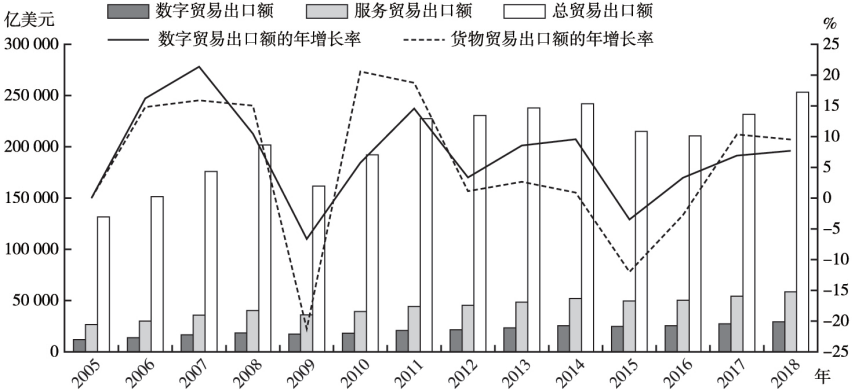
\includegraphics[width=\textwidth]{pic/Fig1.png}
                \vfill
                \begin{center}
                    \footnotesize 图1 \quad 2005-2018年全球数字贸易出口额及其年增长情况
                \end{center}
            \end{column}
            \begin{column}{0.33\textwidth}
                \vfill
                \begin{itemize}
                    \item 数字贸易实现稳定增长
                    \item 相较于其他贸易形式,数字贸易在面对经济危机时表现出更强的“韧性”
                \end{itemize}
                \vfill
            \end{column}
        \end{columns}
        
        \begin{center}
            基于数字交付服务测算出口额作为分析对象,数据来源联合国贸易和发展会议(UNCTAD)
        \end{center}
        \vfill
    }
\end{frame}

\begin{frame}{规制融合}
    \vbox to \textheight{
        \vfill
        \begin{columns}[T]
            \begin{column}{0.66\textwidth}
                \vfill
                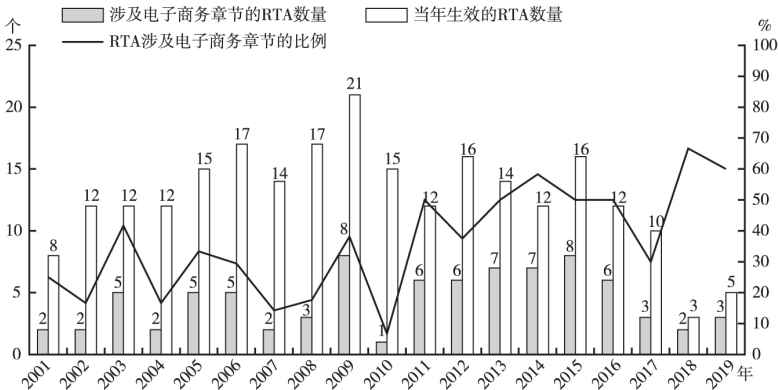
\includegraphics[width=\textwidth]{pic/Fig2.png}
                \vfill
                \begin{center}
                    \footnotesize 图2 \quad 2001-2019年涉及电子商务章节的RTA统计情况
                \end{center}
            \end{column}
            \begin{column}{0.33\textwidth}
                \vfill
                \begin{itemize}
                    \item 2008年全球金融危机发生后,无论是WTO还是RTA都开始逐渐加强对电子商务章节的讨论,规制融合的速度加快
                \end{itemize}
                \vfill
            \end{column}
        \end{columns}

        \begin{center}
            \small 数据来源:WTO网站,网址 \underline{http://rtais.wto.org/UI/PublicSearchByCrResult.aspx}
        \end{center}
        \vfill
    }
\end{frame}

\begin{frame}{规制融合}
    \vbox to \textheight{
        \vfill
        \begin{columns}[T]
            \begin{column}{0.66\textwidth}
                \vfill
                \begin{center}
                    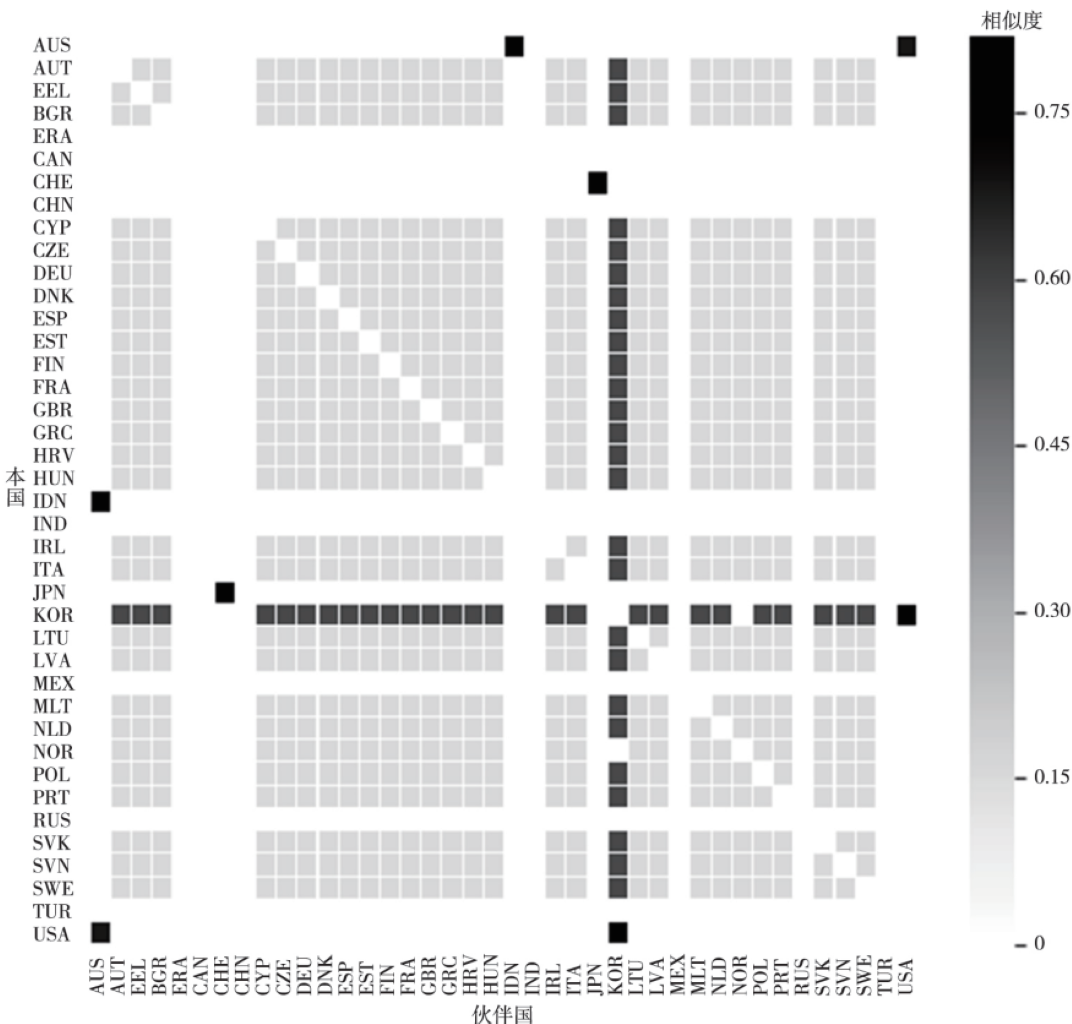
\includegraphics[height=0.5\textheight]{pic/Fig3.png}
                \end{center}

                \vfill
                \begin{center}
                    \footnotesize 图3 \quad 2014年国家间达成数字贸易规则的美式模板相似度统计
                \end{center}
            \end{column}
            \begin{column}{0.33\textwidth}
                \vfill
                \vspace{2.0em}
                \begin{itemize}
                    \item 随着数字贸易规则的标准提高,数字贸易规则出现朝美式模板靠拢的趋势
                \end{itemize}
                \vfill
            \end{column}
        \end{columns}

        \begin{center}
            \small 数据来源:WTO网站,经 Python 脚本处理
        \end{center}
        \vfill
    }
\end{frame}

\subsection{计量模型}
\begin{frame}{计量模型的建立}
    \begin{itemize}
        \item 引力模型
        \begin{footnotesize}
            \begin{gather*}
                RDT_{ijkt} = \beta_0 + \beta_1 Rule_{ijt} + \beta Controls + v_i + v_j + v_k + v_t + \epsilon_{ijkt} \tag{12}
            \end{gather*}
        \end{footnotesize}
        \begin{itemize}
            \item $i, j, k, t$ 分别代表本国,贸易伙伴国,行业和年份
            \item $RDT_{ijkt}$ 被解释变量,国 $i$ 和贸易伙伴国 $j$ 在 $t$ 时期 $k$ 行业的数字贸易额占总贸易额的比重
            \item $Rule_{ijt}$ 解释变量,本国 $i$ 和贸易伙伴国 $j$ 在 $t$ 时期的规制融合水平
            \item $Controls$ 代表控制变量
            \item $v_i, v_j, v_k, v_t$ 分别代表本国固定效应,贸易伙伴国固定效应,行业固定效应和年份固定效应 
            \item $\epsilon_{ijkt}$ 代表随机干扰项
        \end{itemize}
    \end{itemize}
\end{frame}

\begin{frame}{核心指标度量}
    \begin{itemize}
        \item \large 核心被解释变量:数字贸易
        \begin{align*}
            RDT_{ijkt}
        \end{align*}
        \begin{itemize}
            \item $i$ 和 $j$ 国 $k$ 行业 $t$ 时期数字贸易额占总贸易额的比重
            \item 3 个具有数字贸易典型特征行业
            \begin{itemize}
                \item 电影、视频和电视节目制作,录音和音乐出版活动以及节目编制和广播活动
                \item 计算机编程、咨询等相关活动与信息服务活动
                \item 电信业
            \end{itemize}
            \item 4维层面数据,来自 \underline{WIOD 数据库}
            \begin{itemize}
                \item 本国-贸易伙伴国-行业-年份
            \end{itemize}
        \end{itemize}
    \end{itemize}
\end{frame}

\begin{frame}{核心指标度量}
    \begin{itemize}
        \item \large 核心解释变量:规制融合
        \begin{align*}
            Rule_{ijt}
        \end{align*}
        \begin{itemize}
            \item 已签署的RTA是否含有电子商务等数字贸易章节定义经济体之间的规制融合
            \item 如果含有该章节(在生效之后),则取值为1,否则为0
            \begin{itemize}
                \item 1-6月生效的协定算作该年的数字贸易协定
                \item 7-12月生效的协定算作次年的数字贸易协定
            \end{itemize}
            \item “国家对”层面数据,来自 \underline{WTO 官网 RTA 数据库}
        \end{itemize}
    \end{itemize}
\end{frame}

\begin{frame}{控制变量}
    \begin{itemize}
        \item 数据来源:\underline{CEPII 的 Gravity 数据库}
        \begin{enumerate}
            \item 本国、贸易伙伴国国内生产总值($GDP_{it} \text{、} GDP_{jt}$) \\
            \begin{scriptsize} 
                $GDP$ 是引力模型中的关键变量。另外,依据国内市场效应,市场规模的扩大不仅会促进数字贸易的增长,也会促进货物贸易的增长,又由于选取的因变量是数字贸易额占总贸易额的比重,因此系数预期不稳定。
            \end{scriptsize}
            \item 双边地理距离($Dist_{ij}$) \\
            \begin{scriptsize}
                双边地理距离会阻碍国际贸易的开展。同时,Kim et al.(2007) 发现距离在跨境电子商务中有显著负面作用。$Dist_{ij}$ 采用的是加权距离。
            \end{scriptsize}
            \item 是否接壤($Contig_{ij}$) \\
            \begin{scriptsize}
                $Contig_{ij}$ 既代表两国间的空间距离,也可反映文化距离。若两国接壤取值为1,否则为0。
            \end{scriptsize}
            \item 是否具有共同语言($Comlang_{ij}$) \\
            \begin{scriptsize}
                $Comlang_{ij}$ 会降低企业、用户等数字贸易微观参与者的沟通成本,进而促进数字贸易发展。若两国共同官方语言相同则取值为1,否则为0。
            \end{scriptsize}
            \item 是否具有殖民关系($Col_{ij}$) \\
            \begin{scriptsize}
                $Col_{ij}$ 可以反映两国间的制度距离。若两国有殖民关系取值为1,否则为0。
            \end{scriptsize}
        \end{enumerate}
    \end{itemize}
\end{frame}

\begin{frame}{控制变量}
    \begin{itemize}
        \item 数据来源:\underline{Hafstede指数网站(2015年版)}
        \begin{enumerate}
            \item 双边文化距离($DoC_{ij}$) \\
            \begin{scriptsize}
                文化距离、文化偏好等因素也会对国际贸易产生影响。$DoC_{ij}$ 使用 Hofsted 衡量国家文化的6个维度(个人主义、权力差距、不确定性规避、男性价值观、长远利益导向以及放纵主义)得分测算而得,即用这6项指数得分的平均值之差的绝对值作为双边文化距离指标。
            \end{scriptsize}
        \end{enumerate}
        \item 数据来源:\underline{国际电信联盟}
        \begin{enumerate}
            \item 本国和贸易伙伴国互联网水平($Internet_{it}\text{、} Internet_{jt}$) \\
            \begin{scriptsize}
                互联网水平可能会通过影响数字贸易的传输媒介进而影响到数字贸易。互联网水平选用的指标是“个人用户使用互联网的百分比”。
            \end{scriptsize}
        \end{enumerate}
    \end{itemize}
\end{frame}

\section{实证分析}
\subsection{基准回归}
\begin{frame}{基准回归分析}
    \vspace*{-0.8em}
    \begin{columns}[T]
        \begin{column}{0.8\textwidth}
            \scriptsize
            \centering
            \resizebox{\textheight}{!}{ 
                \begin{threeparttable}
                    \caption{基准回归结果}
                    \begin{tabular}{ccccccc}
                        \toprule
                        & \multicolumn{3}{c}{OLS} & \multicolumn{3}{c}{PPML} \\
                        % \cmidrule(lr){2-4} \cmidrule(lr){5-7}
                        & (1) & (2) & (3) & (4) & (5) & (6) \\
                        \midrule
                        $Rule_{ij}$ & 0.0018*** & 0.0024*** & 0.0026*** & 0.2682*** & 0.3544*** & 0.3877*** \\
                        & (0.0002) & (0.0003) & (0.0003) & (0.0294) & (0.0441) & (0.0455) \\
                        $GDP_{it}$ & & -0.0004*** & -0.0004*** & & -0.0539*** & -0.0579*** \\
                        & & (0.0001) & (0.0001) & & (0.0119) & (0.0119) \\
                        $GDP_{jt}$ & & -0.0004*** & -0.0004*** & & -0.0514*** & -0.0660*** \\
                        & & (0.0001) & (0.0001) & & (0.0122) & (0.0117) \\
                        $Dist_{ij}$ & & 0.0007*** & 0.0008*** & & 0.0992*** & 0.1096*** \\
                        & & (0.0001) & (0.0001) & & (0.0190) & (0.0200) \\
                        $Contig_{ij}$ & & -0.0026*** & -0.0027*** & & -0.5080*** & -0.5164*** \\
                        & & (0.0002) & (0.0002) & & (0.0450) & (0.0463) \\
                        $Comlang_{ij}$ & & 0.0059*** & 0.0064*** & & 0.8050*** & 0.8535*** \\
                        & & (0.0008) & (0.0008) & & (0.0766) & (0.0767) \\
                        $Col_{ij}$ & & -0.0020*** & -0.0017*** & & -0.4007*** & -0.3662*** \\
                        & & (0.0003) & (0.0003) & & (0.0615) & (0.0632) \\
                        $DoC_{ij}$ & & & -0.0002*** & & & -0.0309*** \\
                        & & & (0.0001) & & & (0.0107) \\
                        $Internet_{it}$ & & & -0.0002 & & & -0.0390 \\
                        & & & (0.0002) & & & (0.0302) \\
                        $Internet_{jt}$ & & & -0.0003* & & & -0.0503* \\
                        & & & (0.0002) & & & (0.0291) \\
                        常数项 & 0.0064*** & 0.0182*** & 0.0210*** & -5.1082*** & -3.3779*** & -2.8428*** \\
                        & (0.0005) & (0.0028) & (0.0027) & (0.0768) & (0.4228) & (0.4189) \\
                        观测值 & 35 100 & 35 100 & 33 100 & 35 100 & 35 100 & 33 003 \\
                        $R^2$ & 0.0153 & 0.0227 & 0.0238 & 0.0111 & 0.0163 & 0.0164 \\
                        \bottomrule
                    \end{tabular}
                    \begin{tablenotes}
                        \item \textit{说明:} 括号内的值为稳健标准误,* 、**、***分别表示估计系数在 10\% 、5\% 和 1\% 的水平上显著,如未做特殊说明,则所有回归都控制了本国、贸易伙伴国、行业以及年份固定效应,后表同。
                    \end{tablenotes}
                \end{threeparttable}
            }
        \end{column}
        \begin{column}{0.3\textwidth}
            \vspace*{3em}
            \footnotesize
            \begin{itemize}
                \item \uline{
                    普通最小二乘回 \\
                    归(OLS)
                    } \\
                \begin{scriptsize}
                    最基本的回归方法,在经验分析中经常被采用 \\
                    第(1)-(3)列
                \end{scriptsize}
                \item \uline{
                    泊松伪极大似然 \\
                    估计(PPML)
                    } \\
                \begin{scriptsize}
                    适用于因变量存在过多零值的情形 \\
                    第(4)-(6)列
                \end{scriptsize}
            \end{itemize}
        \end{column}
    \end{columns}
\end{frame}

\begin{frame}{基准回归分析}
    \begin{itemize}
        \item 核心解释变量
        \begin{itemize}
            \item 所有回归核心解释变量规制融合的系数均显著为正,\uline{规制融合确实促进了数字贸易}
        \end{itemize}
        \item 控制变量
        \begin{itemize}
            \item 本国和贸易伙伴国国内生产总值系数显著为负,双边地理距离系数显著为正,是否接壤和是否具有殖民关系的系数显著为负,与传统引力模型结论相反 \\
            \begin{scriptsize}
                选取的因变量是数字贸易额占总贸易额的比重,而不是数字贸易额的绝对值,上述控制变量会对传统贸易产生更大影响
            \end{scriptsize}
            \item 是否具有共同语言变量系数显著为正,\uline{共同语言降低了贸易的沟通成本,显著促进了数字贸易}
            \item 双边文化距离显著为负,\uline{文化距离是国家间数字贸易开展的重要障碍}
            \item 本国和贸易伙伴国互联网水平对数字贸易的影响并不稳定 \\
            \begin{scriptsize}
                本国和贸易伙伴国互联网水平对数字贸易和传统贸易会产生同等影响效果
            \end{scriptsize}
        \end{itemize}
    \end{itemize}
\end{frame}

\begin{frame}{稳健性检验}
    \vspace{-0.5cm}
    \begin{columns}[T]
        \begin{column}{0.6\textwidth}
            \tiny
            \setlength{\tabcolsep}{3pt}
            \centering
            \begin{threeparttable}
                \captionsetup{font=tiny}
                \caption{稳健性检验-重新度量数字贸易指标}
                \renewcommand{\arraystretch}{0.8} % 减小行距
                \begin{tabular}{ccc}
                    \toprule
                    & \multicolumn{1}{c}{(1)} & \multicolumn{1}{c}{(1)} \\
                    \midrule
                    $Rule_{ij}$ & 0.5453*** & 0.5142*** \\
                    & (0.0600) & (0.0606) \\
                    $GDP_i$ & 0.8073*** & 0.8047*** \\
                    & (0.0176) & (0.0190) \\
                    $GDP_j$ & 0.8039*** & 0.7995*** \\
                    & (0.0183) & (0.0197) \\
                    $Dist_{ij}$ & -0.6122*** & -0.6266*** \\
                    & (0.0229) & (0.0217) \\
                    $Contig_{ij}$ & -0.4286*** & -0.4269*** \\
                    & (0.0623) & (0.0657) \\
                    $Comlang_{ij}$ & 1.1633*** & 1.1286*** \\
                    & (0.0788) & (0.0885) \\
                    $Col_{ij}$ & -0.1264 & -0.1190 \\
                    & (0.0925) & (0.0932) \\
                    $DoC_{ij}$ & & -0.0313** \\
                    & & (0.0159) \\
                    $Internet_i$ & & -0.0062 \\
                    & & (0.0645) \\
                    $Internet_j$ & & 0.0147 \\
                    & & (0.0607) \\
                    常数项 & -36.5401*** & -36.1791*** \\
                    & (0.7777) & (0.8190) \\
                    观测值 & 35100 & 33003 \\
                    $R^2$ & 0.6220 & 0.6155 \\
                    \bottomrule
                \end{tabular}
            \end{threeparttable}
        \end{column}
        \begin{column}{0.4\textwidth}
            \vspace*{4em}
            \begin{itemize}
                \item 使用数字贸易额作为被解释变量
                \item 规制融合的系数依然显著为正,规制融合对数字贸易具有稳健地促进作用
            \end{itemize}
        \end{column}
    \end{columns}
\end{frame}

\begin{frame}{稳健性检验}
    \vspace*{-0.8em}
    \begin{table}
        \centering
        \caption{更换规制融合指标}
        \label{tab:robustness_check}
        \begin{tabular}{cccc}
            \toprule
            & (1) & (2) & (3) \\
            \midrule
            $RWords_{gt}$ & 0.2045*** & 0.2814*** & 0.2999*** \\
             & (0.0206) & (0.0289) & (0.0293) \\
            控制变量 & 控制 & 控制 & 控制 \\
            观测值 & 35,100 & 35,100 & 33,003 \\
            R$^2$ & 0.0113 & 0.0166 & 0.0167 \\
            \bottomrule
        \end{tabular}
    \end{table}
    \small
    \begin{itemize}
        \item 使用数字贸易条款单词数占总文本单词数的比重($RWords_{ijt}$)代替 $Rule_{ijt}$ 作为核心自变量 \\
        \begin{scriptsize} 
            不同国家间即使达成了同一数字贸易规则,规则内容及其深度也存在一定差异,也就是说规制融合具有异质性,单纯运用虚拟变量方法度量规制融合借粮结果可能并不稳健
        \end{scriptsize}
        \item 核心自变量系数显著为正,规制融合对数字贸易有显著促进作用
    \end{itemize}
\end{frame}

\begin{frame}{内生性问题的讨论与处理}
    \begin{itemize}
        \item 多期倍差法(DID)模型 \\
        \begin{scriptsize}
            控制处理组在虚拟情形下的走势,进而得到规制融合真实的促进效果,从而较好避免政策作为解释变量导致的内生性问题
        \end{scriptsize}
        \begin{gather*}
            RDT_{zt}=\phi_0+\phi_1 DID_{zt}+\phi Controls+v_z+v_t+\epsilon_{zt} \tag{13}
        \end{gather*}
        \begin{itemize}
            \item $DID_{zt}$ 表示因个体而异的处理期虚拟变量
            \begin{itemize}
                \item 若个体 $z$ 在 $t$ 期接受处理代表进入处理期,此后时期均取值为 $1$,否则为 $0$
                \item 等价于处理组虚拟变量 $treat_z$ 和处理期虚拟变量 $post_t$ 的交乘项
            \end{itemize}
            \item $v_z, v_t$ 分别表示个体固定效应和年份固定效应
            \item $\epsilon_{zt}$ 为随机干扰项
        \end{itemize}
    \end{itemize}    
\end{frame}

\begin{frame}{内生性问题的讨论与处理}
    \vspace*{-1em}
    \begin{table}
        \centering
        \caption{多期倍差法(DID)的回归结果}
        \label{tab:DID_results}
        \begin{tabular}{cccc}
            \toprule
            & (1) & (2) & (3) \\
            \midrule
            $DID_{zt}$ & 0.0040*** & 0.0049*** & 0.0053*** \\
            & (0.0003) & (0.0004) & (0.0004) \\
            控制变量 & 控制 & 控制 & 控制 \\
            个体固定效应 & 控制 & 控制 & 控制 \\
            年份固定效应 & 控制 & 控制 & 控制 \\
            观测值 & 35,100 & 35,100 & 33,003 \\
            $R^{2}$ & 0.0060 & 0.0135 & 0.0142 \\
            \bottomrule
        \end{tabular}
    \end{table}
    \begin{itemize}
        \item 规制融合系数显著为正,与基准回归结果保持一致
        \item 交互项系数度量了个体规制融合后超越虚拟情形下的表现,说明规制融合促进了数字贸易的增长
    \end{itemize}
\end{frame}

\begin{frame}{内生性问题的讨论与处理}
    \begin{itemize}
        \item 两阶段最小二乘(2SLS)方法
        \begin{itemize}
            \item DID 方法能缓解样本选择偏差产生的内生性问题,\uline{但不能 \\ 解决模型中的反向因果问题}
        \end{itemize}
        \item 工具变量(IV)方法
        \begin{enumerate}
            \item 两国实现规制融合的概率值
            \begin{itemize}
                \item 根据韩剑等(2019)的研究,设定估计模型:
                \begin{gather*}
                    P(Rule_{ij} = 1 \vert Z)=\alpha_0 \varPhi+\alpha Z
                \end{gather*}
                \item $\varPhi$ 为累计分布函数
                \item $Z$ 为控制变量,包括:双边地理距离、两国的GDP、贸易伙伴之间的类型以及两国的互联网水平
                \item 对模型进行回归,以得到的概率值作为规制融合的工具变量
            \end{itemize}
            \item 两国到赤道距离差取自然对数后的倒数
            \begin{itemize}
                \item 各国到赤道的距离运用的是各国首都到赤道的距离
            \end{itemize}
        \end{enumerate}
    \end{itemize}
\end{frame}

\begin{frame}{内生性问题的讨论与处理}
    \vspace*{-1em}
    \scriptsize
    \centering
    \resizebox{\textwidth}{!}{
        \begin{threeparttable}
            \caption{两阶段最小二乘法的估计结果}
            \label{tab:two_stage_least_squares}
            \begin{tabular}{ccccccc}
                \toprule
                & \makecell[c]{工具变量是 \\ “两国实现 \\ 规制融合的 \\ 概率值”} 
                & \makecell[c]{工具变量是 \\ “两国实现规 \\ 制融合的概 \\ 率值 $\times$ 年份”} 
                & \makecell[c]{工具变量是 \\ “两国到赤道 \\ 距离差取 \\ 自然对数 \\ 后的倒数”} 
                & \makecell[c]{工具变量是 \\ “两国到赤道 \\ 距离差取自 \\ 然对数后的 \\ 倒数 $\times$ 年份”} 
                & \makecell[c]{同时引入 \\ (1) 和 (3) \\ 两个工具 \\ 变量} 
                & \makecell[c]{同时引入 \\ (2) 和 (4) \\ 两个工具 \\ 变量} \\
                & (1) & (2) & (3) & (4) & (5) & (6) \\
                \midrule
                $Rule_{ijt}$ & 0.0102*** & 0.0102*** & 0.0087*** & 0.0087*** & 0.0102*** & 0.0102*** \\
                & (0.0004) & (0.0004) & (0.0017) & (0.0017) & (0.0004) & (0.0004)  \\
                控制变量 & 控制 & 控制 & 控制 & 控制 & 控制 & 控制 \\
                \makecell[c]{Kleibergen-Paap \\ rk LM 统计量} & 5534.5713 & 5521.7264 & 68.9331 & 68.9375 & 5650.6850 & 5637.7088 \\
                & [0.000] & [0.000] & [0.000] & [0.000] & [0.000] & [0.000] \\
                \makecell[c]{Kleibergen-Paap \\ rk Wald F 统计量} & 20525.1132 & 20369.2289 & 300.3013 & 300.4280 & 10426.9758 & 10348.1463 \\
                & \{16.38\} & \{16.38\} & \{16.38\} & \{16.38\} & \{19.93\} & \{19.93\} \\
                \makecell[c]{Hansen-Overid \\ 统计量} & & & & & 0.7286 & 0.7632 \\
                & & & & & [0.3933] & [0.3823] \\
                观测值 & 33,003 & 33,003 & 33,003 & 33,003 & 33,003 & 33,003 \\
                R$^2$  & 0.0069 & 0.0068 & 0.0128 & 0.0128 & 0.0070 & 0.0069 \\
                \bottomrule
            \end{tabular}
            \begin{tablenotes}
                \item {\zhhei 说明:} 小括号内的值为稳健标准误;中括号内的值为相应统计量的 P 值;大括号内的值为 Stock-Yogo 检验 10\%水平上的临界值。Kleibergen-Paap rk LM 统计量检验工具变量与内生变量的相关性,报告的是 LM 统计量及其 P 值,拒绝原假设是合理的;Kleibergen-Paap rk Wald F 统计量检验工具变量是否为弱识别,报告的是 F 统计量及其 10\% 水平下的临界值,超过临界值是合理的。Hansen-Overid 是过度识别检验,报告的是 chi2 统计量及其 P 值,不拒绝原假设是合理的。
            \end{tablenotes}
        \end{threeparttable}
    }
\end{frame}

\begin{frame}{内生性问题的讨论与处理}
    \begin{small}
        \begin{itemize}
            \item \uline{两国实现规制融合的概率值}
            \begin{enumerate}
                \item 双边地理距离等是不同国家实现规制融合考量的重要因素,与规制融合高度相关,满足相关性条件
                \item 仅是一个概率值,不会直接影响数字贸易,满足外生性条件
            \end{enumerate}
            \item \uline{两国到赤道距离差取自然对数后的倒数}
            \begin{enumerate}
                \item 两国到赤道的距离越接近,双边政治关系越融洽,越容易达成国际贸易协定,与规制融合高度相关,满足相关性条件
                \item 各国到赤道距离的差距仅反映政治关系和制度差异,并不会直接影响样本期内经济层面的数字贸易,满足外生性条件
            \end{enumerate}
        \end{itemize}
    \end{small}
    \begin{tcolorbox}[colback=lightyellow,colframe=deepblue,coltext=black]
        \scriptsize
        \begin{itemize}
            \item 规制融合系数显著为正,说明规制融合对数字贸易具有显著促进作用
            \item Kleibergen-Paap rk LM 统计量和 Kleibergen-Paap Wald rk F 统计量结果均拒绝了“工具变量识别不足”和“工具变量弱识别”的零假设,说明本文选取的工具变量是合理的
            \item Hansen-Overid 检验结果无法拒绝原假设,说明工具变量设定有效
        \end{itemize}
    \end{tcolorbox}
\end{frame}


\subsection{机制检验}
\begin{frame}{机制检验}
    \begin{itemize}
        \item 中介效应模型
        \begin{footnotesize}
            \begin{gather*}
                M=\gamma_0+\gamma_1 Rule_{ijt}+\gamma Controls+v_i+v_j+v_k+v_t+\epsilon_{ijkt} \tag{14}
            \end{gather*}
        \end{footnotesize}
        \vspace*{-2em}
        \begin{scriptsize}
            \begin{gather*}
                RDT_{ijkt}=\omega_0+\omega_1 Rule_{ijt}+\omega_2 M+\omega Controls+v_i+v_j+v_k+v_t+\epsilon_{ijkt} \tag{15}
            \end{gather*}
        \end{scriptsize}
        \vspace*{-1em}
        \begin{itemize}
            \item $M$ 为中介效应变量,分别代表贸易成本、双边网络效应和制度距离指标
            \item 中介效应检测,两阶段
            \begin{enumerate}
                \item 基于(14)式运用规制融合对中介变量回归
                \item 基于(15)式将规制融合和中介变量同时引入方程回归
            \end{enumerate}
            \item $\gamma_1$ 与 $\omega_2$ 两系数之积为中介效应,并且 $M$ 作为有效中介变量需满足以下条件
            \begin{enumerate}
                \item (12)式(基准模型)中的系数 $\beta_1$ 显著
                \item $\gamma_1$ 和 $\omega_2$ 至少有 $1$ 个显著
                \item $\beta_1$ 的绝对值大于 $\omega_1$ 的绝对值
            \end{enumerate}
        \end{itemize}
    \end{itemize}
\end{frame}

\begin{frame}{贸易成本的机制检验}
    \begin{itemize}
        \item 简介测度法
        \begin{align*}
            \tau_{ij}=(\frac{x_{ii}x_{jj}}{x_{ij}x_{ji}})^\frac{1}{2(\sigma - 1)}-1 \tag{16}
        \end{align*}
        \begin{itemize}
            \item $\tau_{ij}$ 为 $i$ 和 $j$ 国之间的双边贸易成本
            \item $x_{ii}$ 和 $x_{jj}$ 分别表示 $i$ 和 $j$ 国的国内贸易值
            \item $x_{ij}$ 和 $x_{ji}$ 分别指 $i$ 国向 $j$ 国的出口值和 $j$ 国向 $i$ 国的出口值
            \item $x_{ii}, x_{jj}, x_{ij}, x_{ji}$ 数据来源:WIOD
            \item $\sigma$ 为替代弹性,设定为8
        \end{itemize}
    \end{itemize}
\end{frame}

\begin{frame}{贸易成本的机制检验}
    \begin{columns}[T]
        \begin{column}{0.8\textwidth}
            \centering
            \small
            \begin{threeparttable}
                \captionsetup{font=small}
                \caption{机制检验: 基于贸易成本的中介效应模型}
                \label{tab:mechanism_test}
                \begin{tabular}{c@{\hspace{40pt}}c@{\hspace{40pt}}c}
                    \toprule
                    & 第一阶段 & 第二阶段 \\
                    & 贸易成本 & 数字贸易 \\
                    & (1) & (2) \\
                    \midrule
                    $Rule_{ijt}$ & -0.5632*** & 0.0009** \\
                    & (0.0270) & (0.0004) \\
                    中介变量 &  & -0.0013*** \\
                    & & (0.0003) \\
                    控制变量 & 控制 & 控制 \\
                    观测值 & 29,170 & 29,170 \\
                    $R^2$ & 0.1928 & 0.0422 \\
                    \bottomrule
                \end{tabular}
                \begin{tablenotes}
                    \item {\zhhei 说明}: 本文机制检验部分均使用 OLS 方法回归。  
                \end{tablenotes}
            \end{threeparttable}
        \end{column}
        \begin{column}{0.3\textwidth}
            \vspace*{1.5em}
            \begin{tcolorbox}[colback=lightyellow,colframe=deepblue,coltext=black]
                \begin{footnotesize}
                    第一阶段规制融合和第二阶段贸易成本的系数均显著为负,表明规制融合通过降低贸易成本促进数字贸易的发展
                \end{footnotesize}
            \end{tcolorbox}
        \end{column}
    \end{columns}
\end{frame}

\begin{frame}{双边网络效应的机制检验}
    \begin{itemize}
        \item 囿于数据可得性,无法获知精确的双边网络效用数据
        \item 参考施炳展(2016),运用双边双向网络链接作为替代变量进行中介效用分析,数据来源:Chung(2011)的数据库
        \begin{footnotesize}
            \zhhei
            \item 由于本国和贸易伙伴国的互联网水平与双边网络效应可能存在多重共线性问题,第 (1) 和 (2) 列未添加这两个变量
            \item 为检验回归结果的稳健性,第 (3) 和 (4) 列和基准回归保持一致引入互联网水平和双边网络效应变量
        \end{footnotesize}
    \end{itemize}
    \begin{tcolorbox}[colback=lightyellow,colframe=deepblue,coltext=black]
        \begin{itemize}
            \item 回归结果 \\
            \begin{scriptsize}
                第一阶段规制融合和第二阶段双边网络效应的系数均显著为正,表明规制融合通过增强双边网络效应进而促进数字贸易的发展
            \end{scriptsize}
            \item 稳健性检验结果 \\
            \begin{scriptsize}
                核心变量的回归结果没有发生明显变化
            \end{scriptsize}
        \end{itemize}
    \end{tcolorbox}
\end{frame}

\begin{frame}{双边网络效应的机制检验}
    \vspace{-0.3cm}
    \centering
    \small
    \begin{threeparttable}
        \captionsetup{font=small}
        \caption{机制检验: 基于贸易成本的中介效应模型}
        \begin{tabular}{ccccc}
            \toprule
            & \makecell[c]{第一阶段 \\ 双边网络效应} & \makecell[c]{第二阶段 \\ 数字贸易} & \makecell[c]{第一阶段 \\ 双边网络效应} & \makecell[c]{第二阶段 \\ 数字贸易} \\
            & (1) & (2) & (3) & (4) \\
            \midrule
            $Rule_{ij}$ & 1.8051*** & 0.0073*** & 1.5494*** & 0.0076*** \\
             & (0.4804) & (0.0011) & (0.4967) & (0.0011) \\
            中介变量 & & 0.0001** & & 0.0001** \\
             & & (0.0000) & & (0.0000) \\
            控制变量 & 控制 & 控制 & 控制 & 控制 \\
            观测值 & 2691 & 2691 & 2607 & 2607 \\
            $R^2$ & 0.1997 & 0.0288 & 0.1920 & 0.0298 \\
            \bottomrule
        \end{tabular}
        \begin{tablenotes}
            \item \textbf{说明:} 由于部分样本国家双边双向网络链接数仅有2003和2009年的数据,因此样本观测值发生改变。
        \end{tablenotes}
    \end{threeparttable}
\end{frame}

\begin{frame}{制度距离的机制检验}
    \begin{itemize}
        \item 借鉴黄新飞等(2013),运用14个指标构建了包含政治制度差异、经济制度差异以及制度实施特征差异在内的制度距离指标体系
        \item 运用政治制度和经济制度测算出双边制度距离
        \begin{gather*}
            DOR_{ijt}=\frac{1}{n} \sum_{y=1}^{n} [\frac{(I_{ity}-I_{jty})^2}{V_y}] \tag{17}
        \end{gather*}
        \begin{itemize}
            \item $DOR_{ijt}$ 代表 $t$ 年本国 $i$ 与贸易伙伴国 $j$ 之间的制度距离
            \item $I_{ity}$ 与 $I_{jty}$ 分别表示 $t$ 年 $i$ 与 $j$ 的第 $y$ 项指标和 $j$ 与 $i$ 的第 $y$ 项指标
            \item $V_y$ 是 $y$ 项指标的方差
            \item $n$ 表示指标的总数即 14
        \end{itemize}
        \item 政治领域制度特征,数据来源:世界银行全球治理数据库
        \item 经济领域制度特征,数据来源:美国遗产基金会公布的经济自由度指数
    \end{itemize}
\end{frame}

\begin{frame}{制度距离的机制检验}
    \begin{columns}[T]
        \begin{column}{0.7\textwidth}
            \centering
            \begin{threeparttable}
                \caption{机制检验: 基于制度距离的中介效应模型}
                \begin{tabular}{ccc}
                    \toprule
                    & \makecell[c]{第一阶段 \\ 制度距离} & \makecell[c]{第二阶段 \\ 数字贸易} \\
                    & (1) & (2) \\
                    \midrule
                    $Rule_{ij}$ & -0.5389*** & 0.0026*** \\
                    & (0.0124) & (0.0003) \\
                    中介变量 & & -0.0001 \\
                    & & (0.0001) \\
                    控制变量 & 控制 & 控制 \\
                    观察值 & 33003 & 33003 \\
                    $R^2$ & 0.3570 & 0.0238 \\
                    \bottomrule
                \end{tabular}
            \end{threeparttable}
        \end{column}
        \begin{column}{0.3\textwidth}
            \begin{tcolorbox}[colback=lightyellow,colframe=deepblue,coltext=black]
                第一阶段规制融合的系数显著为负,但第二阶段制度距离系数不显著,规制融合会通过降低制度距离促进数字贸易的发展
            \end{tcolorbox}
        \end{column}
    \end{columns}
\end{frame}

\subsection{扩展分析}
\begin{frame}{基于数字贸易行业的差异性分析}
    \begin{columns}[T]
        \begin{column}{0.7\textwidth}
            \footnotesize
            \centering
            \begin{threeparttable}
                \captionsetup{font=footnotesize}
                \caption{基于行业异质性的回归结果}
                \begin{tabular}{cccc}
                    \toprule
                    & 行业1 & 行业2 & 行业3 \\
                    & (1) & (2) & (3) \\
                    \midrule
                    $Rule_{ijt}$ & $0.8852^{***}$ & $0.1372^{*}$ & $0.4876^{***}$ \\
                    & $(0.1033)$ & $(0.0756)$ & $(0.0526)$ \\
                    控制变量 & 控制 & 控制 & 控制 \\
                    观测值 & 11001 & 11001 & 11001 \\
                    $R^2$ & 0.0422 & 0.0318 & 0.0093 \\
                    \bottomrule
                \end{tabular}
                \begin{tablenotes}
                    \begin{footnotesize}
                        \item {\zhhei 说明:} 行业 1 指电影、视频和电视节目制作、录音和音乐出版活动以及节目编制和广播活动;行业 2 指计算机编程、咨询等相关活动与信息服务活动;行业 3 指电信业务。
                    \end{footnotesize}
                \end{tablenotes}
            \end{threeparttable}
        \end{column}
        \begin{column}{0.4\textwidth}
            \begin{tcolorbox}[colback=lightyellow,colframe=deepblue,coltext=black]
                \footnotesize
                规制融合对“电影、视频和电视节目制作,录音和音乐出版活动以及节目编制和广播活动”行业的数字贸易作用最大且最为显著; 其次是“电信业”; 最后是“计算机编程、咨询等相关活动与信息服务活动”行业
            \end{tcolorbox}
        \end{column}
    \end{columns}
\end{frame}

\begin{frame}{基于美式模板与欧式模板的差异性分析}
    \begin{itemize}
        \item 借鉴韩剑等(2019),计算文本余弦相似度以对数字贸易条款的异质性进行测算
        \item 数字贸易美式模板相似度指标($SimUS_{ijt}$) \\
        \begin{scriptsize}
            所有生效的RTA涉及电子商务章节的条款与TPP(由美国主导的高标准贸易投资规则)进行对比
        \end{scriptsize}
        \item 数字贸易欧式模板相似度指标($SimEU_{ijt}$) \\
        \begin{scriptsize}
            所有生效的RTA涉及电子商务章节的条款与欧洲经济区协议进行对比
        \end{scriptsize}
        \item 数据来源:WTO 的 RTA 数据库中协议文本内容
    \end{itemize}
\end{frame}

\begin{frame}{基于美式模板与欧式模板的差异性分析}
    \vspace*{-2em}
    \begin{center}
        \resizebox{\textwidth}{!}{
            \begin{threeparttable}
                \caption{基于模板异质性的回归结果}
                \begin{tabular}{@{}ccccccc@{}}
                    \toprule
                    & \multicolumn{3}{c}{美式模板相似度} & \multicolumn{3}{c}{欧式模板相似度} \\
                    & (1) & (2) & (3) & (4) & (5) & (6) \\
                    \midrule
                    模板相似度 & $-1.3670^{***}$ & $-2.6701^{***}$ & $-3.2247^{***}$ & $0.7084^{***}$ & $1.3509^{***}$ & $1.6201^{***}$ \\
                    & $(0.2838)$ & $(0.2988)$ & $(0.3083)$ & $(0.1353)$ & $(0.1394)$ & $(0.1458)$ \\
                    控制变量 & 控制 & 控制 & 控制 & 控制 & 控制 & 控制 \\
                    观测值 & 16254 & 16254 & 15069 & 16254 & 16254 & 15069 \\
                    R$^2$ & 0.0177 & 0.0226 & 0.0250 & 0.0114 & 0.0169 & 0.0171 \\
                    \bottomrule
                \end{tabular}
            \end{threeparttable}
        }
    \end{center}
    \vspace*{1em}
    \begin{tcolorbox}[colback=lightyellow,colframe=deepblue,coltext=black]
        \small
        尽管美式模板的标准更高,但相较于欧式模板,美式模板并没有表现出对数字贸易更强的促进作用
    \end{tcolorbox}
\end{frame}


\section{总结}
\begin{frame}{总结}
    \begin{enumerate}
        \item 规制融合有利于促进数字贸易,且在考虑了内生性问题和不同测算指标后,规制融合对数字贸易的促进作用依然稳健。
        \item 规制融合主要通过降低贸易成本,增强双边网络效应和缩短制度距离3条渠道促进数字贸易。
        \item 规制融合对不同数字贸易行业产生的影响存在差异。
        \begin{itemize}
            \item 对“电影、视频和电视节目制作,录音和音乐出版活动以及节目编制和广播活动”行业的数字贸易作用最大
            \item 对“电信业”和“计算机编程、咨询等相关活动与信息服务活动”行业的促进作用相对较小
        \end{itemize}
        \item 尽管美式模板的标准更高,但并没有表现出比欧式模板更强的促进作用。
    \end{enumerate}
\end{frame}

\begin{frame}
    \begin{center}
        {\Huge\calligra Thanks!}
    \end{center}
\end{frame}

\end{document}